\subsection{Results}
\label{sec:results}

\Cref{fig:seq} shows the costs of the final solutions obtained with both approaches in the sequential version. Both follow a linear evolution, but the distinction is clear. As \textbf{Alg1} is used with greater values of $N$, the cost grows at the same rate. With simulated annealing, the cost increases very slowly when compared to $N$. In these results, there is no significant distinction between the two generators.

\begin{figure*}[!htp]
	\centering
	\captionsetup[subfloat]{position=top}
	\subfloat[]{
		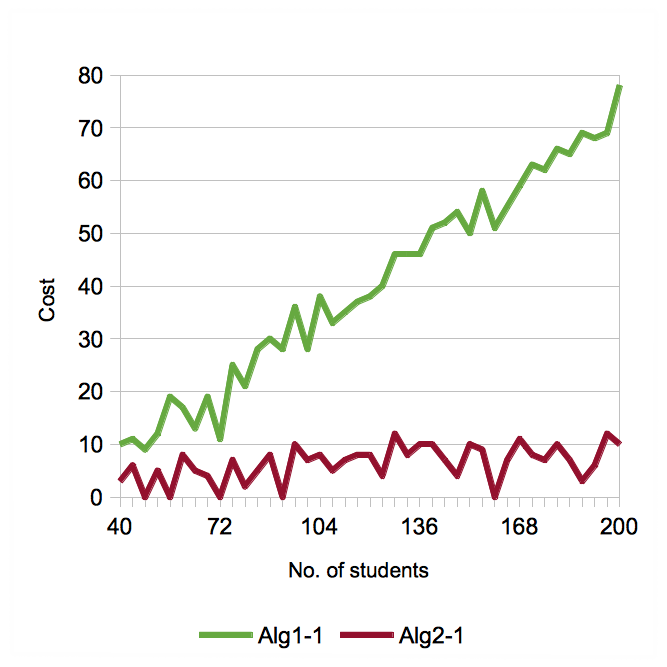
\includegraphics[width=0.45\textwidth]{report/images/rand-01.png}
		\label{fig:seq:rand}
	}
	\hfill
	\subfloat[]{
		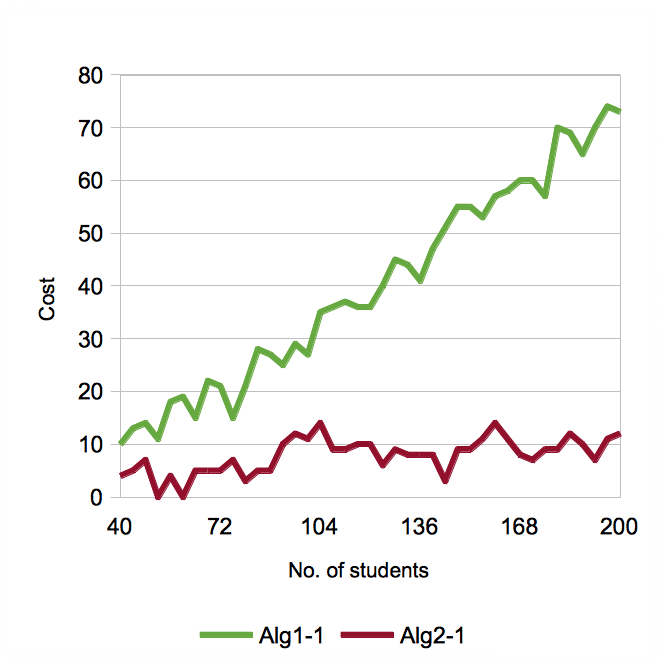
\includegraphics[width=0.45\textwidth]{report/images/arc4-01.png}
		\label{fig:seq:mpi}
	}
	\caption[Sequential Solutions]{Solutions obtained with each approach for the sequential version.\\\subref{fig:seq:rand} used the \texttt{rand} generator; \subref{fig:seq:mpi} used the \texttt{arc4} generator.}
	\label{fig:seq}
\end{figure*}

For the parallel version, \cref{fig:mpi} shows the results for the test with most processes (top) and a midterm (mid). Although the results still follow a similar line, \textbf{Alg1} obtained slightly better solutions in parallel, being this more noticeable in the top case. As for \textbf{Alg2}, the mid case already shows a clear improvement, and the top case obtains the perfect solution most of the times for the values chosen for $N$.

In the parallel version there is also a diference between the two generators. In both cases, the \texttt{rand} generator succeded in achieving the perfect solution more times than the \texttt{arc4}. Yet, the \texttt{arc4} generator follows a very low and constant line of results, while the \texttt{rand} generator is very irregular in the mid case, where it obtained values near the sequential results when it did not manage to find the perfect solution. Comparing both approaches, this version amplifies the distinction already present in the sequential version.

\begin{figure*}[!htp]
	\centering
	\captionsetup[subfloat]{position=top}
	\subfloat[]{
		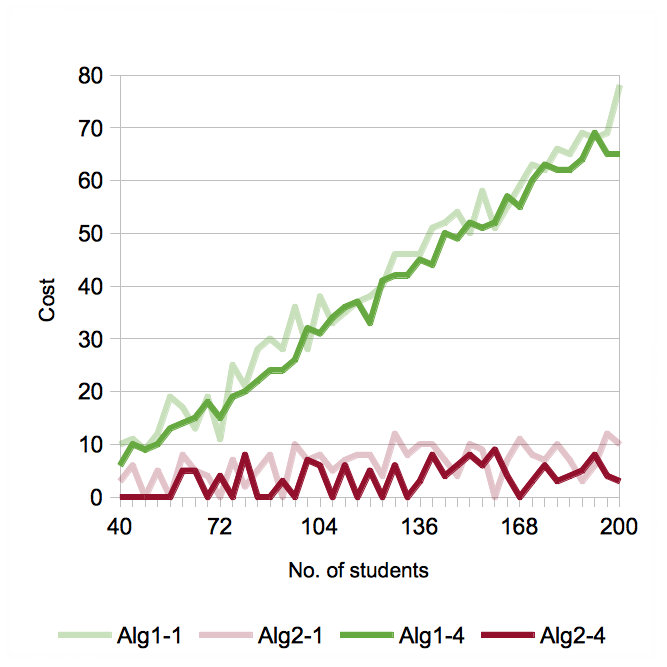
\includegraphics[width=0.45\textwidth]{report/images/rand-04.png}
		\label{fig:mpi:rand:04}
	}
	\hfill
	\subfloat[]{
		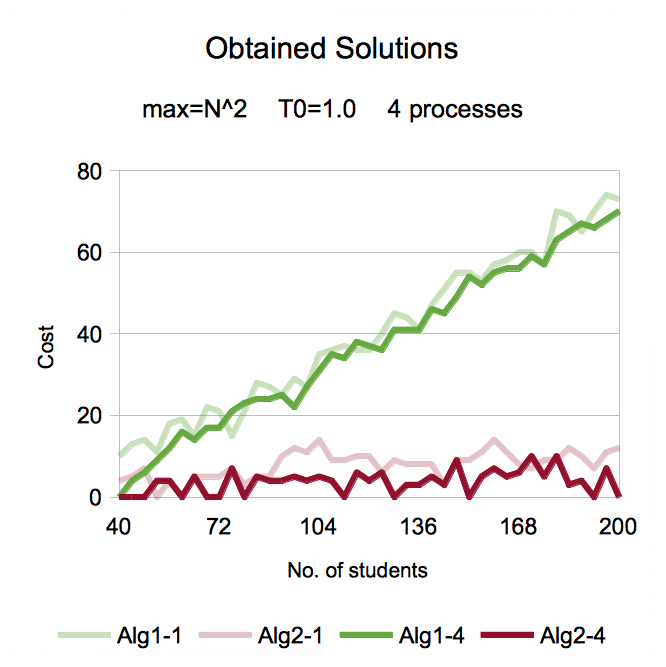
\includegraphics[width=0.45\textwidth]{report/images/arc4-04.png}
		\label{fig:mpi:arc4:04}
	}

	\captionsetup[subfloat]{position=bottom}
	\subfloat[]{
		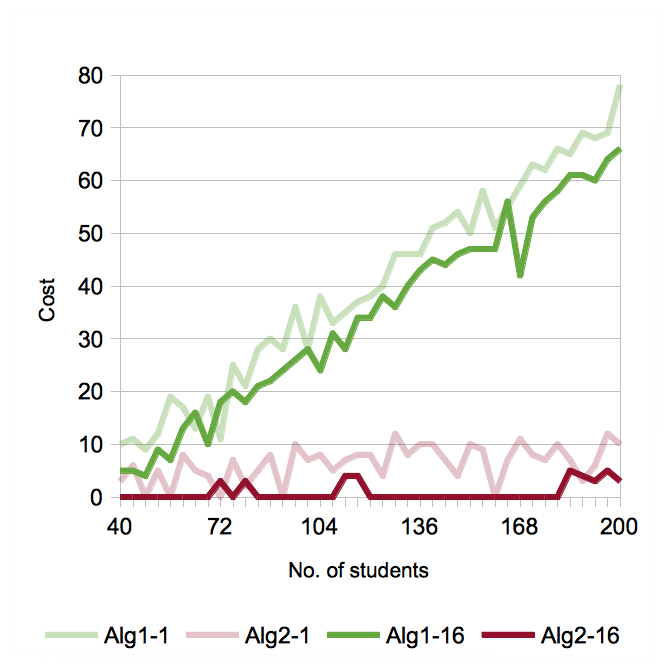
\includegraphics[width=0.45\textwidth]{report/images/rand-16.png}
		\label{fig:mpi:rand:16}
	}
	\hfill
	\subfloat[]{
		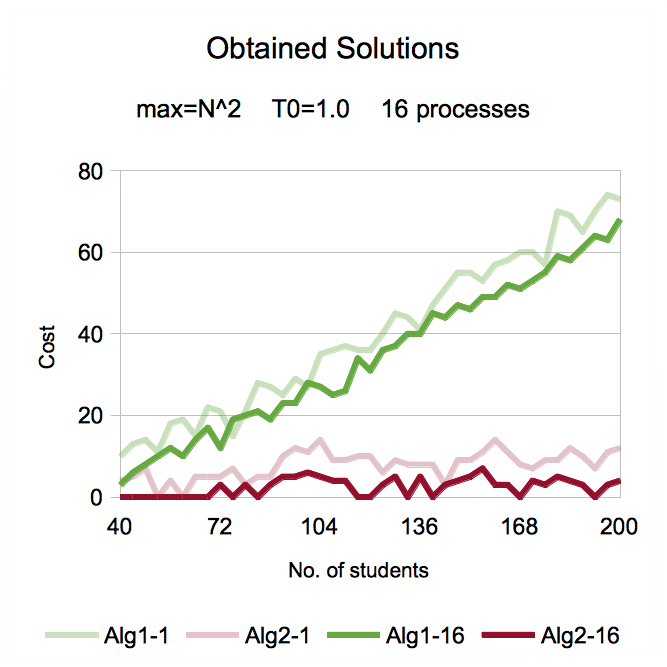
\includegraphics[width=0.45\textwidth]{report/images/arc4-16.png}
		\label{fig:mpi:arc4:16}
	}
	\caption[Parallel Solutions]{Solutions obtained with each approach for the two generators using the parallel version.\\\subref{fig:mpi:rand:04} and \subref{fig:mpi:arc4:04} were obtained using 4 processes; \subref{fig:mpi:rand:16} and \subref{fig:mpi:arc4:16} were obtained using 16 processes.\\\subref{fig:mpi:rand:04} and \subref{fig:mpi:rand:16} used the \texttt{rand} generator; \subref{fig:mpi:arc4:04} and \subref{fig:mpi:arc4:16} used the \texttt{arc4} generator.}
	\label{fig:mpi}
\end{figure*}